%%%%%%%%%%%%%%%%%%%%%%%%%%%%%%%%%%%%%%%%%
% Short Sectioned Assignment
% LaTeX Template
% Version 1.0 (5/5/12)
%
% This template has been downloaded from:
% http://www.LaTeXTemplates.com
%
% Original author:
% Frits Wenneker (http://www.howtotex.com)
%
% License:
% CC BY-NC-SA 3.0 (http://creativecommons.org/licenses/by-nc-sa/3.0/)
%
%%%%%%%%%%%%%%%%%%%%%%%%%%%%%%%%%%%%%%%%%

%----------------------------------------------------------------------------------------
%	PACKAGES AND OTHER DOCUMENT CONFIGURATIONS
%----------------------------------------------------------------------------------------

\documentclass[paper=a4, fontsize=11pt]{scrartcl} % A4 paper and 11pt font size

\usepackage[T1]{fontenc} % Use 8-bit encoding that has 256 glyphs
%\usepackage{fourier} % Use the Adobe Utopia font for the document - comment this line to return to the LaTeX default
\usepackage[english]{babel} % English language/hyphenation
\usepackage{amsmath,amsfonts,amsthm} % Math packages
\usepackage{mathtools} %More math! (For dscases)
\usepackage{hyperref} %HTML package
\usepackage{pgfplots} %Makes plots in LaTeX
\usepackage{tikz} %Also tikz?
\usepackage{bm} %makes vectors bold
\usepackage{bbm} %Blackboard bold 1
\usepgfplotslibrary{fillbetween}%Let's me fill between named plots
\usepackage{graphicx} %import pics
\graphicspath{ {Python_figs/} }
\DeclareGraphicsExtensions{.pdf,.png,.jpg}
\usepackage{sectsty} % Allows customizing section commands
\allsectionsfont{ \normalfont\scshape} % Make all sections the default font and small caps


\renewcommand{\thesubsection}{\alph{subsection}} %Make subsections start with letters

\usepackage{fancyhdr} % Custom headers and footers
\pagestyle{fancyplain} % Makes all pages in the document conform to the custom headers and footers
\fancyhead{} % No page header - if you want one, create it in the same way as the footers below
\fancyfoot[L]{} % Empty left footer
\fancyfoot[C]{} % Empty center footer
\fancyfoot[R]{\thepage} % Page numbering for right footer
\renewcommand{\headrulewidth}{0pt} % Remove header underlines
\renewcommand{\footrulewidth}{0pt} % Remove footer underlines
\setlength{\headheight}{13.6pt} % Customize the height of the header

\numberwithin{equation}{section} % Number equations within sections (i.e. 1.1, 1.2, 2.1, 2.2 instead of 1, 2, 3, 4)
\numberwithin{figure}{section} % Number figures within sections (i.e. 1.1, 1.2, 2.1, 2.2 instead of 1, 2, 3, 4)
\numberwithin{table}{section} % Number tables within sections (i.e. 1.1, 1.2, 2.1, 2.2 instead of 1, 2, 3, 4)

\setlength\parindent{0pt} % Removes all indentation from paragraphs - comment this line for an assignment with lots of text

\usepackage{listings}
\lstset{language=Python}
%----------------------------------------------------------------------------------------
%	TITLE SECTION
%----------------------------------------------------------------------------------------

\newcommand{\horrule}[1]{\rule{\linewidth}{#1}} % Create horizontal rule command with 1 argument of height

\title{	Assignment 11}

\author{Benjamin Jakubowski} % Your name

\date{\normalsize\today} % Today's date or a custom date

\begin{document}

\maketitle % Print the title

%----------------------------------------------------------------------------------------
%	PROBLEM 1
%----------------------------------------------------------------------------------------

\section{Convexity}

\subsection{Sum of convex functions is convex}

$f := \sum_{i=1}^m a_if_i$ is a convex function if the constants $a_1, \dots, a_m$ are nonnegative. \\

Proof:\\

Let $x, y \in \mathbb{R}, \theta \in (0,1)$ be given. Then
\begin{align*}
\theta f(x) + (1-\theta)f(y) &= \theta \sum_{i=1}^m a_i f_i(x) + (1-\theta)\sum_{i=1}^ma_if_i(y) \\ 
   &= \sum_{i=1}^m a_i \left( \theta f_i(x) + (1-\theta)f_i(y)\right) \\
   &\geq \sum_{i=1}^m a_i f_i\left(\theta x + (1-\theta)y\right) \qquad{} \text{(since every $f_i$ is convex)}  \\
   &= f\left(\theta x + (1-\theta)y\right)
\end{align*}
So $\theta f(x) + (1-\theta)f(y) \geq f\left(\theta x + (1-\theta)y\right)$ and $f$ is convex. \qed

\subsection{Maximum of convex functions is convex}

Now let
\[g(x) = \max_{1 \leq i \leq m} f_i(x)\]
We show $g(x)$ is itself convex. Again, let $x, y \in \mathbb{R}$ be given. Now let
\[i_x = \arg \max_{1 \leq i \leq m} f_i(x)\]
\[i_y = \arg \max_{1 \leq i \leq m} f_i(y)\]

Then
\[
\theta g(x) + (1-\theta)g(y) = \theta f_{i_x}(x) + (1-\theta)f_{i_y}(y)
\]

So now, let $i$ be given. Then note
\begin{align*}
f_{i_x}(x) \geq f_i(x) \qquad{} & \qquad{} f_{i_y}(y)\geq f_i(y) \\
\iff \theta f_{i_x}(x) \geq \theta f_i(x) \qquad{} & \qquad{} (1-\theta) f_{i_y}(y)\geq (1-\theta) f_i(y) \\
\implies \theta f_{i_x}(x) + (1-\theta) f_{i_y}(y) &\geq \theta f_i(x) + (1-\theta) f_i(y)
\end{align*}

Thus, 
\begin{align*}
\theta g(x) + (1-\theta)g(y) &= \theta f_{i_x}(x) + (1-\theta)f_{i_y}(y) \\
   &\geq \theta f_i(x) + (1-\theta) f_i(y) \qquad \text{for all $ i, 1\leq i \leq m$}
\end{align*}

Next since $f_i$ is convex, for any $i$
\[\theta f_i(x) + (1-\theta)f_i(y) \geq f_i(\theta x + (1-\theta)y)\]

Hence, for all $i, 1 \leq i \leq m$,
\begin{align*}
\theta g(x) + (1-\theta) g(y) &= \theta f_{i_x}(x) + (1-\theta)f_{i_y}(y) \\
   &\geq \theta f_i(x) + (1-\theta) f_i(y) \\
   &\geq f_i\left(\theta x + (1-\theta)y\right)
\end{align*}

But then, in particular,
\begin{align*}
\theta g(x) + (1-\theta) g(y) &\geq \max_{1 \leq i \leq m}  f_i\left(\theta x + (1-\theta)y\right) \\
   &= g\left(\theta x + (1-\theta)y\right)
\end{align*}

So $g$ is convex. \qed

\subsection{Product of convex functions not necessarily convex}

Let $h := \prod_{i=1}^m f_i$. We aim to show that $h$ is not necessarily convex.\\

Let $f_1 = x^2 - 5x$. Note $f_1$ is convex since $f_1''(x) = 2 > 0 \text{ for all } x$.\\
Let $f_2 = x^2 + 5x$. Note $f_2$ is convex since $f_2''(x) = 2 > 0 \text{ for all } x$.

Now,
\begin{align*}
h(x) &= f_1(x)f_2(x) \\
   &= (x^2 - 5x)(x^2 + 5x) \\ 
   &= x^4 - 25x^2
\end{align*}
So $h''(x) = 12x^2 - 50 < 0 \text{ if } |x| \leq \sqrt{\frac{50}{12}}$.
Hence, $h$ is not convex.


%----------------------------------------------------------------------------------------
%	PROBLEM 2
%----------------------------------------------------------------------------------------

\section{Implementing 1D optimization algorithms}

Here is the code added to implement derivative descent and Newton's method.

\begin{lstlisting}[frame=single, basicstyle=\small]

def derivative_descent(x_ini, f, der_f, step, eps=0.01):
    x_i = x_ini
    der_f_at_x = der_f(x_i)
    path = [x_i]
    while np.abs(der_f_at_x) > eps:
        x_i = x_i - step*der_f(x_i)
        path.append(x_i)
        der_f_at_x = der_f(x_i)
    return np.array(path)

def newton_method(x_ini, f, der_f, der2_f, eps=0.01):
    x_i = x_ini
    der_f_at_x = der_f(x_i)
    path = [x_i]
    while np.abs(der_f_at_x) > eps:
        x_i = x_i - der_f(x_i)/der2_f(x_i)
        path.append(x_i)
        der_f_at_x = der_f(x_i)
    return np.array(path)
    
def quadratic_approx(x, point, f, df, d2f):
    approx = f(point) + df(point)*(x-point)\
    + 1.0/2.0 * d2f(point)*(x-point)**2.0
    return approx

\end{lstlisting}


%----------------------------------------------------------------------------------------
%	PROBLEM 3
%----------------------------------------------------------------------------------------

\section{Projected gradient descent}

\subsection{Projection onto positive orthant $\mathbb{R}_+^n$}

Take $\bm{x} \in \mathbb{R}^n$. We can represent this vector using the standard basis as
\[\bm{x} = \sum_{i=1}^n \alpha_i \bm{e}_i\]

Now, if $\alpha_i \geq 0$ for all $i, 1 \leq i \leq n$, then $\bm{x} \in \mathbb{R}_+^n$, so $\mathcal{P}_{\mathbb{R}_+^n} \bm{x} = \bm{x}$. \\

If not, then let
\[
\tilde{\alpha}_i =
\begin{cases}
0 & \text{ if } \alpha_i \leq 0 \\
\alpha_i & \text{ otherwise }
\end{cases}
\]
Then
\[\mathcal{P}_{\mathbb{R}_+^n} \bm{x} = \sum_{i=1}^n \tilde{\alpha}_i \bm{e}_i\]

To see this is in fact the projection onto the positive orthant, consider that:
\begin{align*}
\mathcal{P}_{\mathbb{R}_+^n} \bm{x} &= \arg \min_{\bm{u} \in \mathbb{R}_+^n} ||\bm{x} - \bm{u}||_2^2 \\
   &= \arg \min_{\bm{u} \in \mathbb{R}_+^n} \sum_{i=1}^n (x_i - u_i)^2
\end{align*}
Now take an arbitrary $i$. There are two cases to consider:
\begin{itemize}
\item If $x_i > 0$, $\arg \min_{u_i \in R_+} (x_i - u_i) = x_i$.
\item If $x_i \leq 0$, $\arg \min_{u_i \in R_+} (x_i - u_i) = 0$.
\end{itemize}

But this is exactly how we defined the projection:
\[\mathcal{P}_{\mathbb{R}_+^n} \bm{x} = \sum_{i=1}^n \tilde{\alpha}_i \bm{e}_i\]

\subsection{Projection onto the unit $\ell_2$ ball}

Take $\bm{x} \in \mathbb{R}^n$. First, note that if $||\bm{x}||_2 \leq 1, \mathcal{P}_{\mathcal{B}_{\ell_2}} \bm{x} = \bm{x}$. \\`

If not, then 
\[\mathcal{P}_{\mathcal{B}_{\ell_2}} \bm{x} = \frac{\bm{x}}{||\bm{x}||_2} \]

We can see this is in fact the projection by noting $\mathcal{P}_{\mathcal{B}_{\ell_2}} \bm{x}$ is also the projection of $\bm{x}$ onto the hyperplane tangent to the surface of $\mathcal{B}_{\ell_2}$ at $\frac{\bm{x}}{||\bm{x}||_2}$. This immediately implies that the distance between $\bm{x}$ and any other vector in $\mathcal{B}_{\ell_2}$ must be greater than $\mathcal{P}_{\mathcal{B}_{\ell_2}} \bm{x}$.\\

(To see this, note this distance is the norm of a vector, call it $\bm{z}$. If $\bm{z}$ passes through the tangent hyperplane at some point other than $\frac{\bm{x}}{||\bm{x}||_2}$, then the norm of $\bm{z}$ is greater than $||\bm{x} - \mathcal{P}_{\mathcal{B}_{\ell_2}} \bm{x}||_2$, so our alternate candidate  cannot be the projection).

\subsection{Implementing projected gradient descent}

Here is the code added to $hw11\_pb3.py$ to implement projected gradient descent:
\begin{lstlisting}[frame=single, basicstyle=\small]
def projected_gradient_descent(x_ini,f,grad,step,eps,proj,n_iter):
    x_i = proj(x_ini)
    path = [x_i]
    grad_at_x = grad(x_i)
    iterations = 1
    while np.sqrt(np.dot(grad_at_x, grad_at_x)) > eps\
    and iterations <= n_iter:
        x_i = x_i - step*grad(x_i)
        x_i = proj(x_i)
        path.append(x_i)
        grad_at_x = grad(x_i)
        iterations +=1
    return np.array(path)

def projection_positive(x):
    func = lambda x_i: (0 if x_i<0 else x_i)
    v_func = np.vectorize(func)
    proj = v_func(x)
    return proj

def projection_l2(x):
    if np.linalg.norm(x)<=1:
        return x
    else:
        return x/(np.linalg.norm(x))
\end{lstlisting}

The figures are:

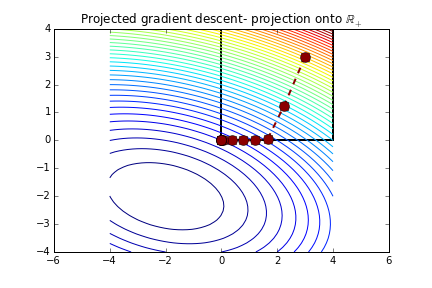
\includegraphics[scale = 1]{Q3Ci.png}

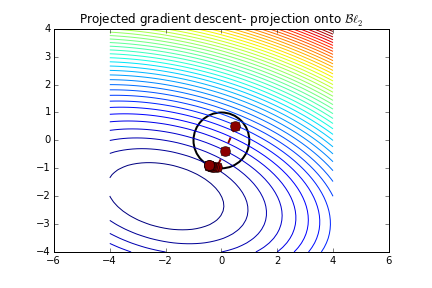
\includegraphics[scale = 1]{Q3Cii.png}

\subsection{Intuitive justification for optimal point in constraint set}

The intuitive justification that the algorithm reaches the optimal point is based on the observation that the final solution (reached after 10 iterations) appears to be at the lowest point within the set. We can see this in the contour lines/level sets- in both cases (i.e. constrained to $\mathbb{R}_+$ and to $\mathcal{B}_{\ell_2}$) the final solution is at or below the lowest level set  depicted in the contour plot.
%----------------------------------------------------------------------------------------
\end{document}